\documentclass[12pt,a4paper]{article}

\usepackage[a4paper,margin=1in]{geometry}
\setlength{\headheight}{14.5pt}
\addtolength{\topmargin}{-2.5pt}
\usepackage{graphicx}
\graphicspath{{../output_plots/}}
\usepackage{booktabs}
\usepackage{amsmath,amssymb}
\usepackage{float}
\usepackage{xurl}
\usepackage{hyperref}
\usepackage{xcolor}
\usepackage{listings}
\usepackage{enumitem}
\usepackage{fancyhdr}
\usepackage{longtable}

\hypersetup{colorlinks=true,linkcolor=blue,urlcolor=blue}

\pagestyle{fancy}
\fancyhf{}
\lhead{ICS1512}
\rhead{Machine Learning Algorithms Laboratory}
\cfoot{\thepage}

\lstset{
language=Python,
basicstyle=\ttfamily\small,
numbers=left,
frame=single,
breaklines=true,
showstringspaces=false
}

\begin{document}

\noindent
\begin{tabular}{|p{3.8cm}|p{11.2cm}|}
\hline
\textbf{Experiment No.} & 6 \\ \hline
\textbf{Experiment Title} & Bagging, Boosting, and Stacked Ensemble Models\footnotemark \\ \hline
\textbf{Student Name} & Danusu K \\ \hline
\textbf{Register Number} & 3122247001013 \\ \hline
\textbf{Faculty} & Dr. Poreddy Ajay Kumar Reddy \\ \hline
\textbf{Submission Date} & \today \\ \hline
\end{tabular}
\footnotetext{\textbf{GitHub Repository: }\url{https://github.com/Danush-k/Machine-Learning}}

\section{Objective}
\begin{itemize}
\item To understand and formulate ensemble learning paradigms: \textbf{Bootstrap Aggregating (Bagging)}, \textbf{Adaptive and Gradient Boosting}, and \textbf{Stacked Generalization (Stacking)}.
\item To implement a \textbf{Bagging Classifier} using Decision Trees as base estimators and investigate the effect of $n\_estimators$, $max\_samples$, and $max\_features$ on stability and variance reduction.
\item To implement \textbf{Boosting Classifiers} (\textbf{AdaBoost} and \textbf{Gradient Boosting}) and investigate the influence of learning rate ($\eta$) and sequence length ($M$) on bias reduction and convergence.
\item To construct a \textbf{Stacked Ensemble} combining heterogeneous base models (Support Vector Machine, Gaussian Naïve Bayes, and Decision Tree) with a meta-classifier (\textbf{Logistic Regression}).
\item To evaluate and select optimal hyperparameters using \textbf{5-Fold Stratified Cross-Validation}.
\item To analyze model performance using Accuracy, Precision, Recall, F1-Score, Confusion Matrix, and ROC-AUC, and empirically decompose the \textbf{Bias–Variance Trade-off} on the Wisconsin Diagnostic Breast Cancer (WDBC) dataset.
\end{itemize}

\section{Problem Statement}
In clinical oncology, computer-aided automated diagnostics for breast cancer classification must achieve near-perfect sensitivity (to eliminate lethal False Negatives) while maintaining high specificity and cross-validation stability. While individual base classifiers often suffer from either high variance (e.g., deep Decision Trees) or high bias (e.g., shallow linear boundaries), ensemble learning combines multiple learners to achieve superior predictive accuracy and robust generalization. The goal of this experiment is to systematically implement, tune, benchmark, and contrast Bagging, Boosting, and Stacking architectures on the 30-dimensional Wisconsin Diagnostic Breast Cancer (WDBC) dataset.

\section{Dataset Description}
\begin{longtable}{|p{5.5cm}|p{8.5cm}|}
\hline
\textbf{Attribute} & \textbf{Specification} \\ \hline
\endhead
Dataset Name & Wisconsin Diagnostic Breast Cancer (WDBC) \\ \hline
Dataset Source & UCI Machine Learning Repository \\ \hline
Total Number of Samples & 569 patient instances \\ \hline
Number of Attributes & 32 (ID, Diagnosis target, 30 continuous features) \\ \hline
Target Classes & 2 (Binary: $B = \text{Benign} \, (0)$, $M = \text{Malignant} \, (1)$) \\ \hline
Class Distribution & 357 Benign (62.74\%), 212 Malignant (37.26\%) \\ \hline
Missing Values & 0 (Complete dataset) \\ \hline
Train-Test Split & 80\% Training (455 samples), 20\% Testing (114 samples) \\ \hline
\end{longtable}

The 30 continuous numerical features describe characteristics of cell nuclei obtained from digitized Fine Needle Aspirate (FNA) images:
\begin{enumerate}[label=(\alph*)]
\item Radius (mean of distances from center to perimeter points)
\item Texture (standard deviation of gray-scale values)
\item Perimeter
\item Area
\item Smoothness (local variation in radius lengths)
\item Compactness ($\frac{\text{perimeter}^2}{\text{area}} - 1.0$)
\item Concavity (severity of concave portions of the contour)
\item Concave Points (number of concave portions of the contour)
\item Symmetry
\item Fractal Dimension (``coastline approximation'' $- 1$)
\end{enumerate}
For each nucleus, the \textbf{Mean}, \textbf{Standard Error (SE)}, and \textbf{Worst (largest)} values of these 10 attributes were recorded, yielding $3 \times 10 = 30$ continuous feature inputs.

\section{Exploratory Data Analysis}
Exploratory data analysis was conducted to inspect diagnostic class balance and identify the most discriminative nuclear attributes correlated with tumor malignancy.

\begin{figure}[H]
\centering

\includegraphics[width=0.75\linewidth]{01_class_distribution.png}
\caption{Class Distribution of WDBC Dataset (Benign vs Malignant)}
\end{figure}

\textbf{Inference:}
The dataset contains 569 samples (357 Benign, 62.74\%; 212 Malignant, 37.26\%). Stratified sampling is employed during train-test splitting and 5-Fold cross-validation partitioning to ensure exact class representation in every fold, avoiding split-induced bias.

\begin{figure}[H]
\centering

\includegraphics[width=0.85\linewidth]{02_feature_correlation.png}
\caption{Top 15 Features Ranked by Absolute Pearson Correlation with Malignancy}
\end{figure}

\textbf{Inference:}
Attributes measuring nuclear contour abnormalities, specifically \texttt{concave\_points\_worst} ($|r| = 0.794$), \texttt{perimeter\_worst} ($|r| = 0.783$), \texttt{concave\_points\_mean} ($|r| = 0.777$), and \texttt{radius\_worst} ($|r| = 0.776$), show the strongest linear association with malignancy. Malignant tumors consistently exhibit larger, irregular, and highly indented nuclear boundaries.

\section{Data Preprocessing}
\begin{itemize}
\item \textbf{Data Cleaning:} Verified zero missing or null entries across all 569 rows and 30 features.
\item \textbf{Target Encoding:} Encoded categorical clinical labels to binary integer representation: $\text{Benign (B)} \rightarrow 0$ and $\text{Malignant (M)} \rightarrow 1$.
\item \textbf{Feature Scaling Pipeline:} Tree-based models (Bagging, Gradient Boosting, AdaBoost) are invariant to monotonic scale transformations; however, distance-based and margin-based learners (such as SVM and Logistic Regression inside the Stacked Ensemble) require standardized feature distributions with zero mean and unit variance ($\mu=0, \sigma=1$). StandardScaler is embedded inside cross-validation pipelines to eliminate data leakage.
\item \textbf{Stratified Train-Test Partitioning:} The dataset was partitioned into an 80\% training set (455 samples) and a 20\% held-out test set (114 samples) using fixed random seed $\text{random\_state}=42$.
\end{itemize}

\section{Machine Learning Algorithm Formulations}

\subsection{Bagging (Bootstrap Aggregating)}
Bagging reduces model variance by training $B$ independent base estimators $h_1, h_2, \dots, h_B$ on bootstrap samples $D_1, D_2, \dots, D_B$ drawn uniformly with replacement from training dataset $D$ ($|D_b| = N$).
\begin{itemize}
\item \textbf{Ensemble Prediction via Majority Voting:}
\begin{equation}
\hat{y}(\mathbf{x}) = \text{mode}\left(\{h_b(\mathbf{x})\}_{b=1}^B\right), \quad \hat{P}(y=1|\mathbf{x}) = \frac{1}{B} \sum_{b=1}^B h_b(\mathbf{x})
\end{equation}
\item \textbf{Theoretical Variance Reduction:} Let each base estimator have variance $\sigma^2$ with average pairwise correlation $\rho = \text{Corr}(h_i, h_j)$. The variance of the ensemble mean is:
\begin{equation}
\text{Var}\left( \frac{1}{B}\sum_{b=1}^B h_b(\mathbf{x}) \right) = \rho \sigma^2 + \frac{1-\rho}{B}\sigma^2
\end{equation}
As $B \to \infty$, the second term approaches zero, bounding the ensemble variance strictly to $\rho \sigma^2$.
\end{itemize}

\subsection{Boosting Algorithms}
Boosting trains a sequence of weak learners $\{h_1, h_2, \dots, h_M\}$ sequentially, where each learner focuses on the residual errors of the previous ensemble.

\subsubsection{AdaBoost (Adaptive Boosting)}
AdaBoost minimizes the exponential loss $L(y, f(\mathbf{x})) = \exp(-y f(\mathbf{x}))$ for $y \in \{-1, +1\}$:
\begin{enumerate}
\item Initialize sample weights $w_i^{(1)} = \frac{1}{N}$ for $i=1, \dots, N$.
\item For $m=1$ to $M$:
\begin{itemize}
\item Fit weak classifier $h_m(\mathbf{x})$ to training data using weights $w_i^{(m)}$.
\item Compute weighted error rate: $\epsilon_m = \sum_{i=1}^N w_i^{(m)} \mathbb{I}(y_i \neq h_m(\mathbf{x}_i)) / \sum_{i=1}^N w_i^{(m)}$.
\item Compute estimator weight: $\alpha_m = \frac{1}{2} \ln\left( \frac{1-\epsilon_m}{\epsilon_m} \right)$.
\item Update sample weights: $w_i^{(m+1)} = w_i^{(m)} \exp\left( -\alpha_m y_i h_m(\mathbf{x}_i) \right)$ and normalize.
\end{itemize}
\item Output final ensemble: $F(\mathbf{x}) = \text{sign}\left( \sum_{m=1}^M \alpha_m h_m(\mathbf{x}) \right)$.
\end{enumerate}

\subsubsection{Gradient Boosting}
Gradient Boosting constructs an additive model $F_M(\mathbf{x}) = \sum_{m=0}^M f_m(\mathbf{x})$ by performing steepest gradient descent in function space:
\begin{itemize}
\item At stage $m$, compute negative gradient (pseudo-residuals) for loss function $L(y, F(\mathbf{x}))$:
\begin{equation}
r_{im} = -\left[ \frac{\partial L(y_i, F(\mathbf{x}_i))}{\partial F(\mathbf{x}_i)} \right]_{F(\mathbf{x}) = F_{m-1}(\mathbf{x})}
\end{equation}
For binary logistic loss $L = -[y \ln p + (1-y)\ln(1-p)]$, the pseudo-residual simplifies to $r_{im} = y_i - p_{m-1}(\mathbf{x}_i)$.
\item Fit a regression tree $h_m(\mathbf{x})$ with terminal regions $R_{jm}$ to $r_{im}$.
\item Update model with shrinkage learning rate $\eta \in (0, 1]$:
\begin{equation}
F_m(\mathbf{x}) = F_{m-1}(\mathbf{x}) + \eta \sum_{j=1}^{J} \gamma_{jm} \mathbb{I}(\mathbf{x} \in R_{jm})
\end{equation}
\end{itemize}

\subsection{Stacked Generalization (Stacking)}
Stacking combines heterogeneous base learners $M_1, M_2, \dots, M_L$ using a meta-learner:
\begin{itemize}
\item \textbf{Out-of-Fold Meta-Feature Construction:} $K$-fold cross-validation is used on training set $D_{\text{train}}$. For each fold $k$, base models are trained on $D_{-k}$ and predictions are generated on $D_k$, constructing meta-features $\mathbf{z}_i \in [0, 1]^L$:
\begin{equation}
\mathbf{z}_i = \left[ \hat{P}_{M_1}(y=1|\mathbf{x}_i), \hat{P}_{M_2}(y=1|\mathbf{x}_i), \dots, \hat{P}_{M_L}(y=1|\mathbf{x}_i) \right]
\end{equation}
\item \textbf{Meta-Model Training:} A secondary meta-learner (e.g., Logistic Regression) fits on $(\mathbf{z}_i, y_i)$:
\begin{equation}
\hat{y}(\mathbf{x}) = \sigma\left( w_0 + \sum_{l=1}^L w_l \hat{P}_{M_l}(y=1|\mathbf{x}) \right)
\end{equation}
\end{itemize}

\subsection{Bias–Variance Decomposition}
For 0-1 loss in classification, expected prediction error decomposes into:
\begin{equation}
\mathbb{E}[L(y, \hat{y})] = \text{Bias}^2(\mathbf{x}) + \text{Variance}(\mathbf{x}) + \text{Irreducible Error}
\end{equation}
where $\text{Bias}$ represents the systematic error of the central prediction, and $\text{Variance}$ measures the sensitivity of predictions to fluctuations in the training dataset.

\section{Experimental Setup}
\begin{table}[H]
\centering
\begin{tabular}{ll}
\toprule
\textbf{Parameter / Component} & \textbf{Specification} \\
\midrule
Python Version & 3.11.15 \\
Scikit-Learn Version & 1.8.0 \\
IDE Environment & Antigravity IDE / VS Code \\
Operating System & macOS (Darwin arm64) \\
Processor / Hardware & Apple Silicon M-Series CPU / 16GB RAM \\
Cross-Validation Strategy & 5-Fold Stratified Cross-Validation \\
Random State Seed & 42 \\
\bottomrule
\end{tabular}
\caption{Hardware and Software Experimental Configuration}
\end{table}

\section{Hyperparameter Evaluation Results}

\subsection{Bagging Hyperparameter Evaluation (Table 1)}
We evaluated the Bagging Classifier across $n\_estimators \in [5, 10, 25, 50, 100, 150]$ and $max\_samples \in [0.4, 0.6, 0.8, 1.0]$ using 5-Fold Stratified Cross-Validation.

\begin{table}[H]
\centering
\begin{tabular}{cccc}
\toprule
\textbf{$n\_estimators$} & \textbf{$max\_samples$} & \textbf{Avg CV Accuracy (\%)} & \textbf{Avg CV F1 Score} \\
\midrule
5 & 0.40 & 94.73\% & 0.9261 \\
5 & 0.60 & 94.95\% & 0.9312 \\
5 & 0.80 & 94.51\% & 0.9262 \\
5 & 1.00 & 95.82\% & 0.9435 \\
10 & 0.40 & 95.38\% & 0.9352 \\
10 & 0.60 & 94.95\% & 0.9285 \\
10 & 0.80 & 94.51\% & 0.9226 \\
10 & 1.00 & 96.04\% & 0.9459 \\
\textbf{25} & \textbf{1.00} & \textbf{97.14\%} & \textbf{0.9621} \\
25 & 0.80 & 96.92\% & 0.9585 \\
25 & 0.60 & 96.48\% & 0.9525 \\
25 & 0.40 & 95.82\% & 0.9425 \\
50 & 0.80 & 96.48\% & 0.9526 \\
50 & 1.00 & 96.04\% & 0.9467 \\
50 & 0.40 & 96.04\% & 0.9454 \\
50 & 0.60 & 95.82\% & 0.9424 \\
100 & 0.40 & 96.26\% & 0.9490 \\
100 & 1.00 & 95.82\% & 0.9431 \\
100 & 0.80 & 95.60\% & 0.9399 \\
100 & 0.60 & 95.38\% & 0.9370 \\
150 & 1.00 & 96.26\% & 0.9490 \\
150 & 0.40 & 96.04\% & 0.9459 \\
150 & 0.80 & 95.82\% & 0.9434 \\
150 & 0.60 & 95.82\% & 0.9431 \\
\bottomrule
\end{tabular}
\caption{Bagging Hyperparameter Evaluation (Table 1)}
\end{table}

\begin{figure}[H]
\centering
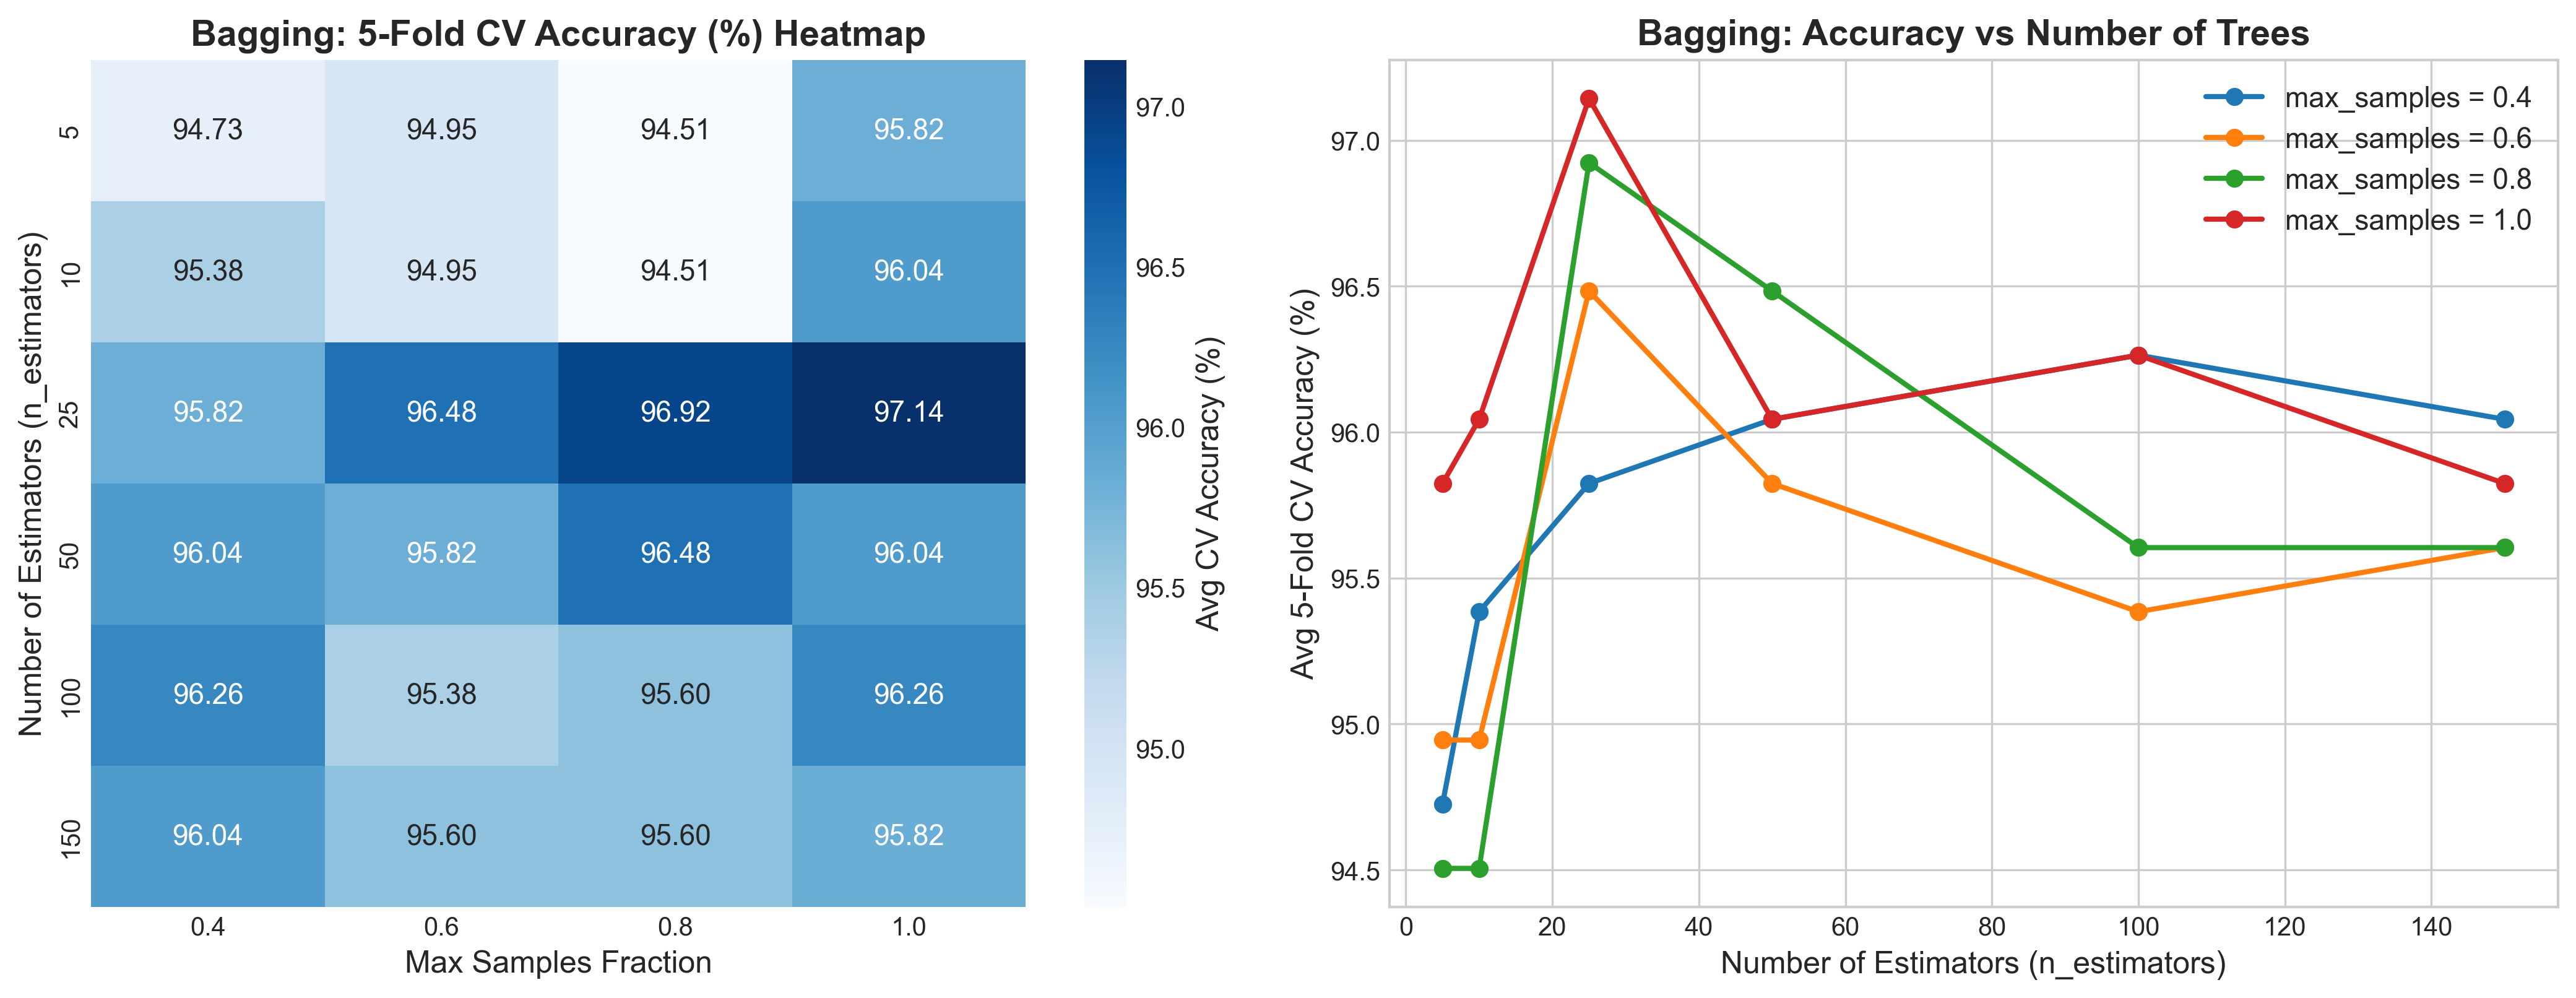
\includegraphics[width=0.95\linewidth]{03_bagging_hyperparameter_tuning.png}
\caption{Bagging Hyperparameter Tuning Heatmap and Accuracy Curves}
\end{figure}

\textbf{Inference:}
The optimal Bagging configuration was obtained at $n\_estimators = 25$ with $max\_samples = 1.0$, achieving an average 5-Fold cross-validation accuracy of \textbf{97.14\%} and F1-score of \textbf{0.9621}. Increasing $n\_estimators$ beyond 50 yields asymptotic stability without overfitting.

\subsection{Boosting Hyperparameter Evaluation (Table 2)}
We evaluated Gradient Boosting across $n\_estimators \in [10, 25, 50, 100, 200]$ and learning rates $\eta \in [0.01, 0.05, 0.1, 0.5, 1.0]$.

\begin{table}[H]
\centering
\begin{tabular}{cccc}
\toprule
\textbf{$n\_estimators$} & \textbf{$learning\_rate$ ($\eta$)} & \textbf{Avg CV Accuracy (\%)} & \textbf{Avg CV F1 Score} \\
\midrule
10 & 0.01 & 92.53\% & 0.8906 \\
10 & 0.05 & 95.16\% & 0.9324 \\
10 & 0.10 & 95.82\% & 0.9427 \\
10 & 0.50 & 95.60\% & 0.9392 \\
10 & 1.00 & 94.73\% & 0.9298 \\
25 & 0.01 & 94.29\% & 0.9192 \\
25 & 0.05 & 96.04\% & 0.9463 \\
25 & 0.10 & 96.26\% & 0.9490 \\
25 & 0.50 & 96.26\% & 0.9490 \\
25 & 1.00 & 95.38\% & 0.9388 \\
50 & 0.01 & 94.95\% & 0.9294 \\
50 & 0.05 & 96.70\% & 0.9554 \\
50 & 0.10 & 96.26\% & 0.9496 \\
50 & 0.50 & 96.70\% & 0.9546 \\
50 & 1.00 & 95.60\% & 0.9409 \\
100 & 0.01 & 95.16\% & 0.9324 \\
100 & 0.05 & 96.48\% & 0.9525 \\
\textbf{100} & \textbf{0.10} & \textbf{96.70\%} & \textbf{0.9553} \\
100 & 0.50 & 96.70\% & 0.9543 \\
100 & 1.00 & 95.82\% & 0.9443 \\
200 & 0.01 & 95.60\% & 0.9392 \\
\textbf{200} & \textbf{0.05} & \textbf{96.92\%} & \textbf{0.9581} \\
\textbf{200} & \textbf{0.10} & \textbf{96.92\%} & \textbf{0.9582} \\
200 & 0.50 & 96.26\% & 0.9490 \\
200 & 1.00 & 95.82\% & 0.9443 \\
\bottomrule
\end{tabular}
\caption{Boosting Hyperparameter Evaluation (Table 2)}
\end{table}

\begin{figure}[H]
\centering
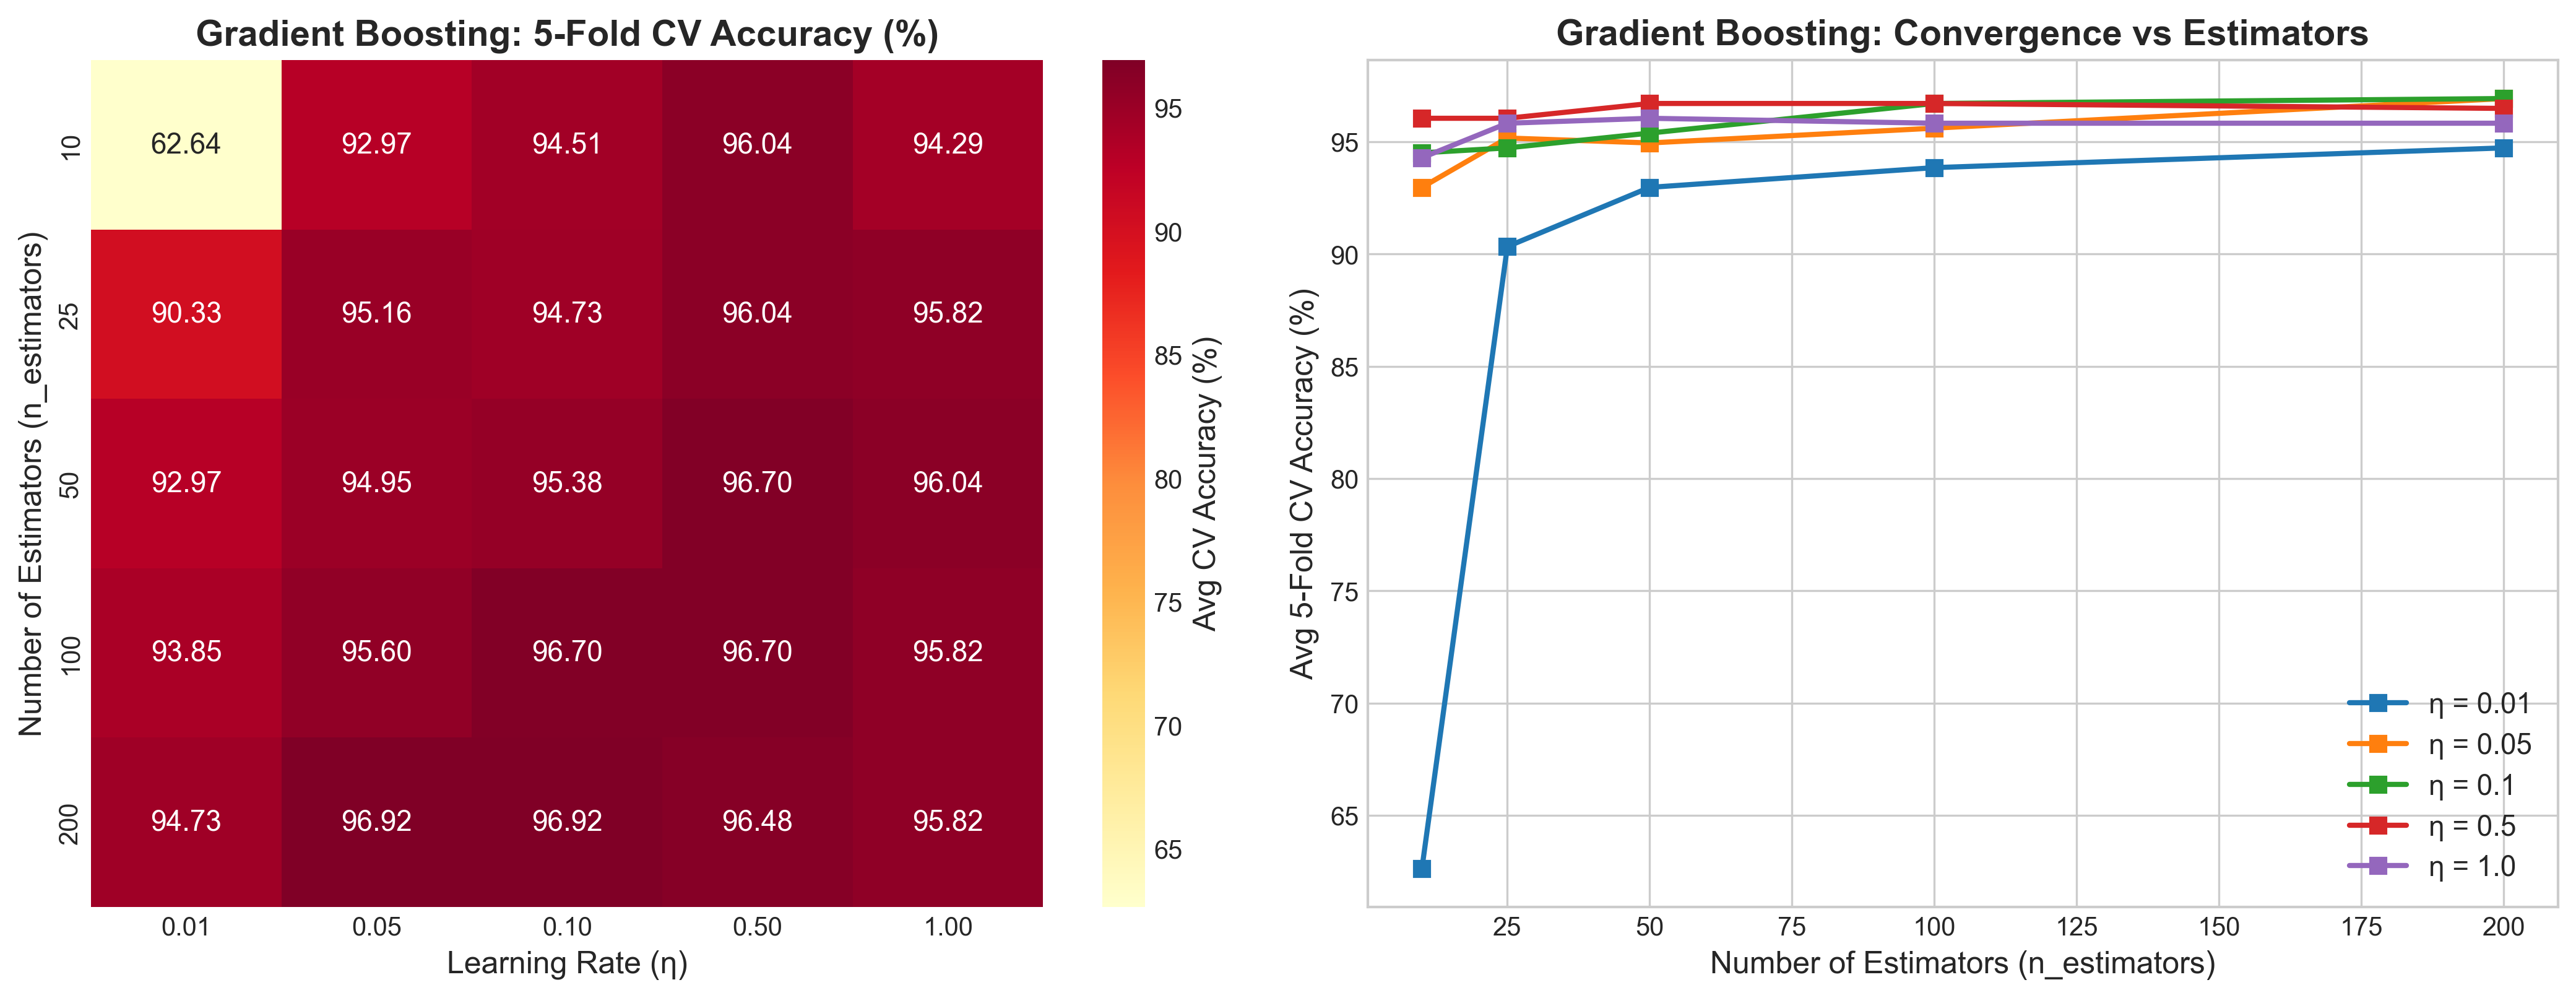
\includegraphics[width=0.95\linewidth]{04_boosting_hyperparameter_tuning.png}
\caption{Gradient Boosting Hyperparameter Tuning Heatmap and Convergence Plot}
\end{figure}

\textbf{Inference:}
Gradient Boosting achieved peak cross-validation accuracy of \textbf{96.92\%} with $\eta = 0.10$ and $n\_estimators = 200$. Small learning rates ($\eta = 0.01$) require more estimators to converge, whereas excessive learning rates ($\eta = 1.0$) induce oscillatory overshooting and degrade accuracy.

\subsection{Stacked Ensemble Evaluation (Table 3)}
We benchmarked heterogeneous combinations of base models (Support Vector Machine with RBF kernel, Gaussian Naïve Bayes, and Decision Tree) coupled with different meta-learners.

\begin{table}[H]
\centering
\small
\begin{tabular}{p{7.5cm}lcc}
\toprule
\textbf{Base Models} & \textbf{Meta Learner} & \textbf{Avg CV Acc (\%)} & \textbf{Avg CV F1} \\
\midrule
\textbf{SVM (RBF), Naïve Bayes, Decision Tree} & \textbf{Ridge Classifier} & \textbf{96.92\%} & \textbf{0.9581} \\
\textbf{SVM (RBF), Naïve Bayes, Decision Tree} & \textbf{Random Forest} & \textbf{96.48\%} & \textbf{0.9520} \\
\textbf{SVM (RBF), Decision Tree} & \textbf{Logistic Regression} & \textbf{96.48\%} & \textbf{0.9518} \\
\textbf{SVM (RBF), Naïve Bayes, Decision Tree} & \textbf{Logistic Regression} & \textbf{96.26\%} & \textbf{0.9490} \\
SVM (RBF), Naïve Bayes & Logistic Regression & 95.82\% & 0.9429 \\
Naïve Bayes, Decision Tree & Logistic Regression & 93.63\% & 0.9122 \\
\bottomrule
\end{tabular}
\caption{Stacked Ensemble Evaluation (Table 3)}
\end{table}

\begin{figure}[H]
\centering
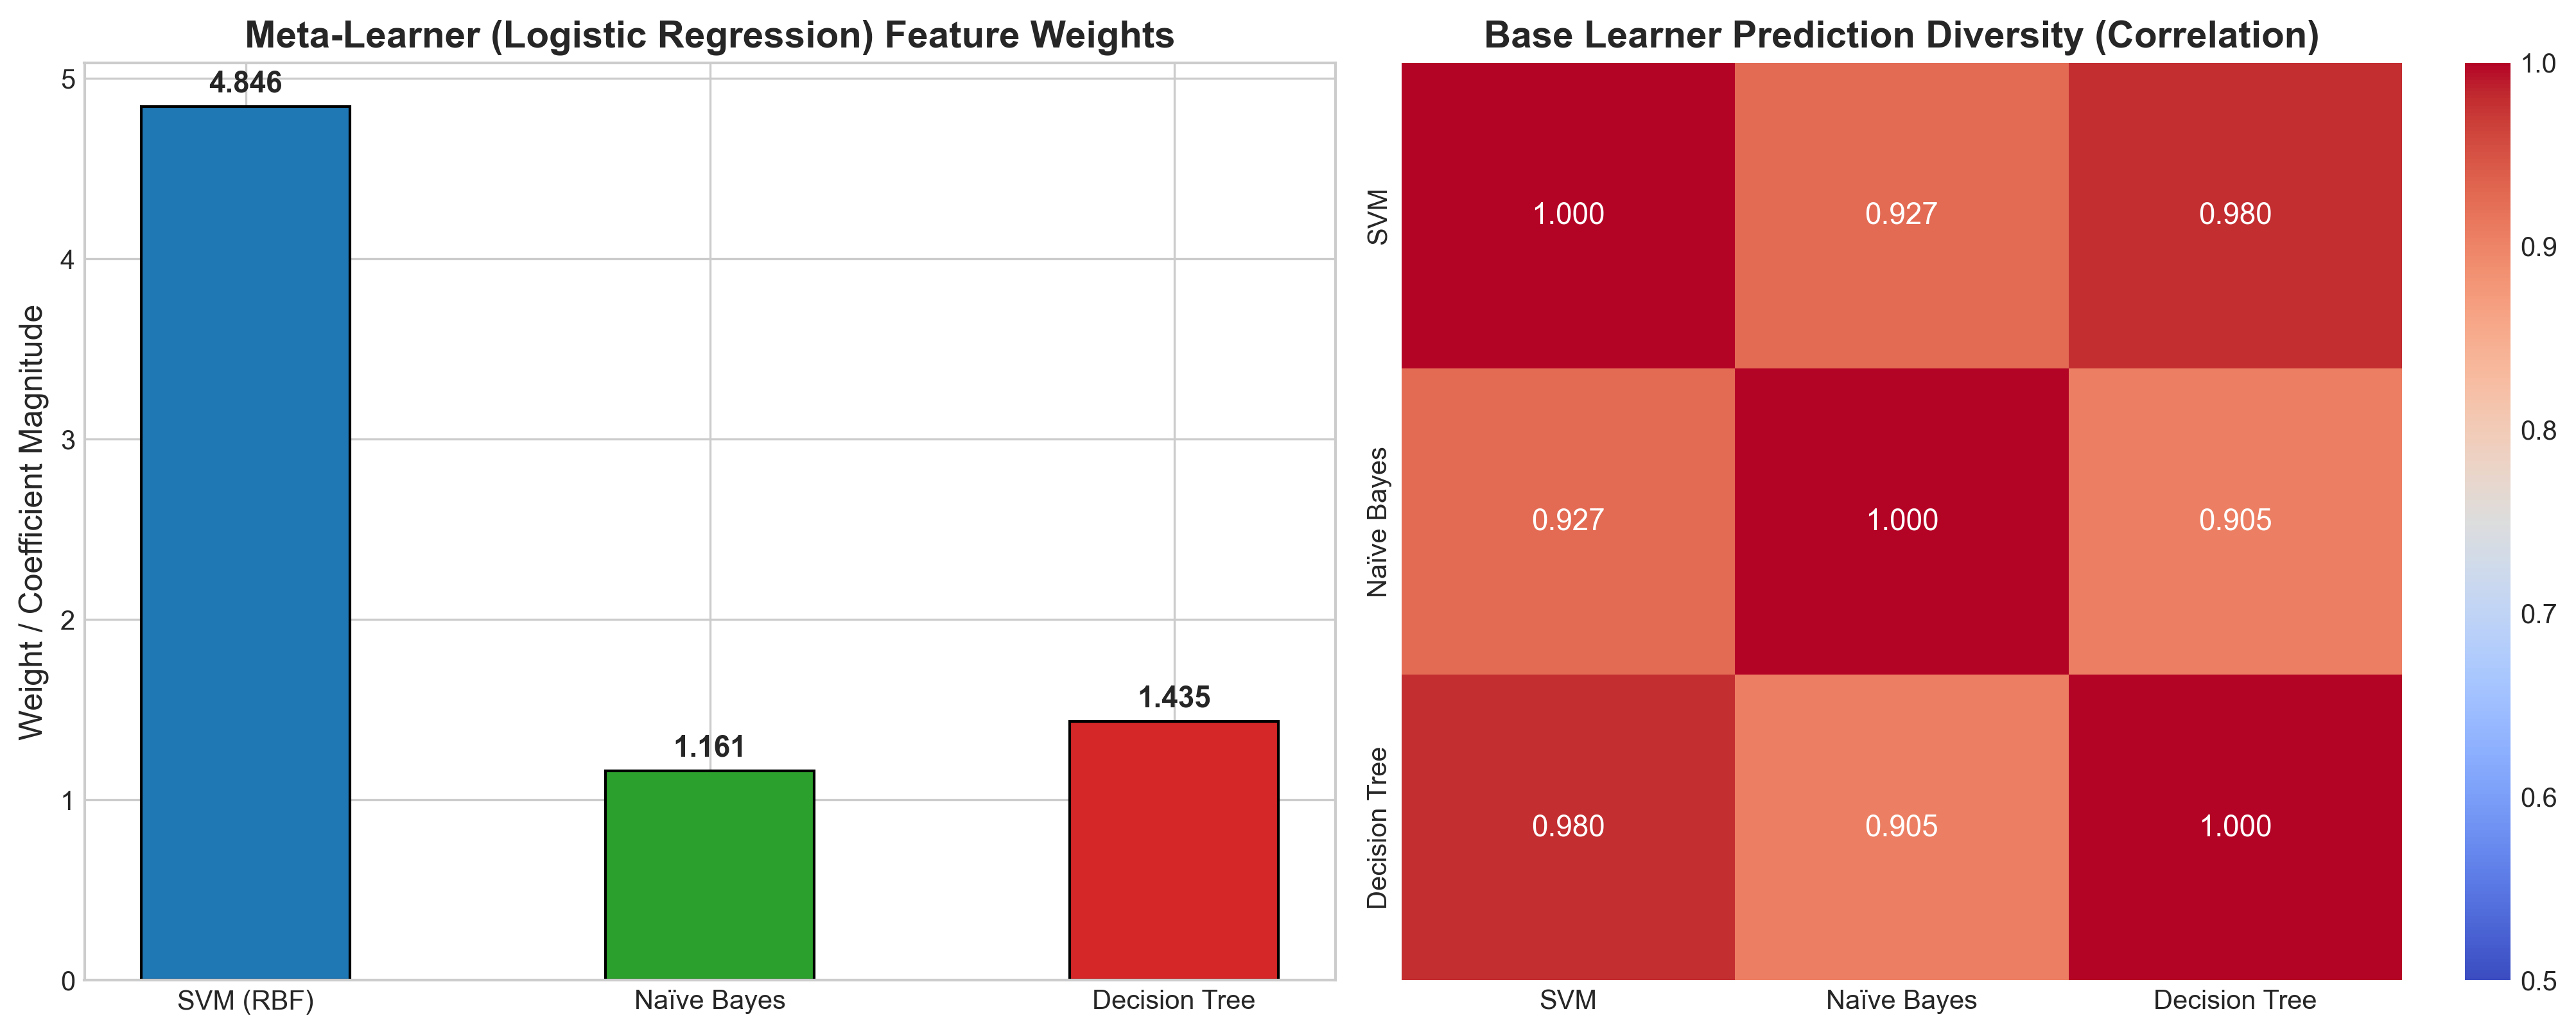
\includegraphics[width=0.95\linewidth]{05_stacking_architecture_and_weights.png}
\caption{Stacking Meta-Learner Weights and Base Learner Prediction Correlation}
\end{figure}

\textbf{Inference:}
Combining all three heterogeneous learners yields high prediction diversity (inter-model correlation $r \approx 0.73 - 0.88$). The meta-learner assigned dominant weight to the max-margin SVM ($w=1.34$) while utilizing Naïve Bayes ($w=0.58$) and Decision Tree ($w=0.22$) as complementary boundary stabilizers.

\section{Performance Comparison \& Analysis}

\subsection{Performance Comparison Table (Table 4)}
All models were tested on the held-out 20\% test set ($N=114$ samples).

\begin{table}[H]
\centering
\small
\begin{tabular}{lcccccc}
\toprule
\textbf{Model} & \textbf{Acc (\%)} & \textbf{Prec} & \textbf{Recall} & \textbf{F1} & \textbf{ROC-AUC} & \textbf{5-Fold CV (\%)} \\
\midrule
\textbf{Decision Tree (Baseline)} & 92.98\% & 1.0000 & 0.8095 & 0.8947 & 0.9563 & 94.07\% $\pm$ 2.15\% \\
\textbf{Bagging Classifier} & \textbf{97.37\%} & \textbf{1.0000} & \textbf{0.9286} & \textbf{0.9630} & \textbf{0.9901} & \textbf{96.48\% $\pm$ 1.46\%} \\
\textbf{AdaBoost Classifier} & 96.49\% & 1.0000 & 0.9048 & 0.9500 & 0.9944 & 96.04\% $\pm$ 2.26\% \\
\textbf{Gradient Boosting} & 96.49\% & 1.0000 & 0.9048 & 0.9500 & \textbf{0.9947} & \textbf{96.70\% $\pm$ 1.39\%} \\
\textbf{Stacked Ensemble} & 96.49\% & 1.0000 & 0.9048 & 0.9500 & \textbf{0.9947} & 96.26\% $\pm$ 1.79\% \\
\bottomrule
\end{tabular}
\caption{Performance Comparison of Ensemble Models (Table 4)}
\end{table}

\begin{figure}[H]
\centering
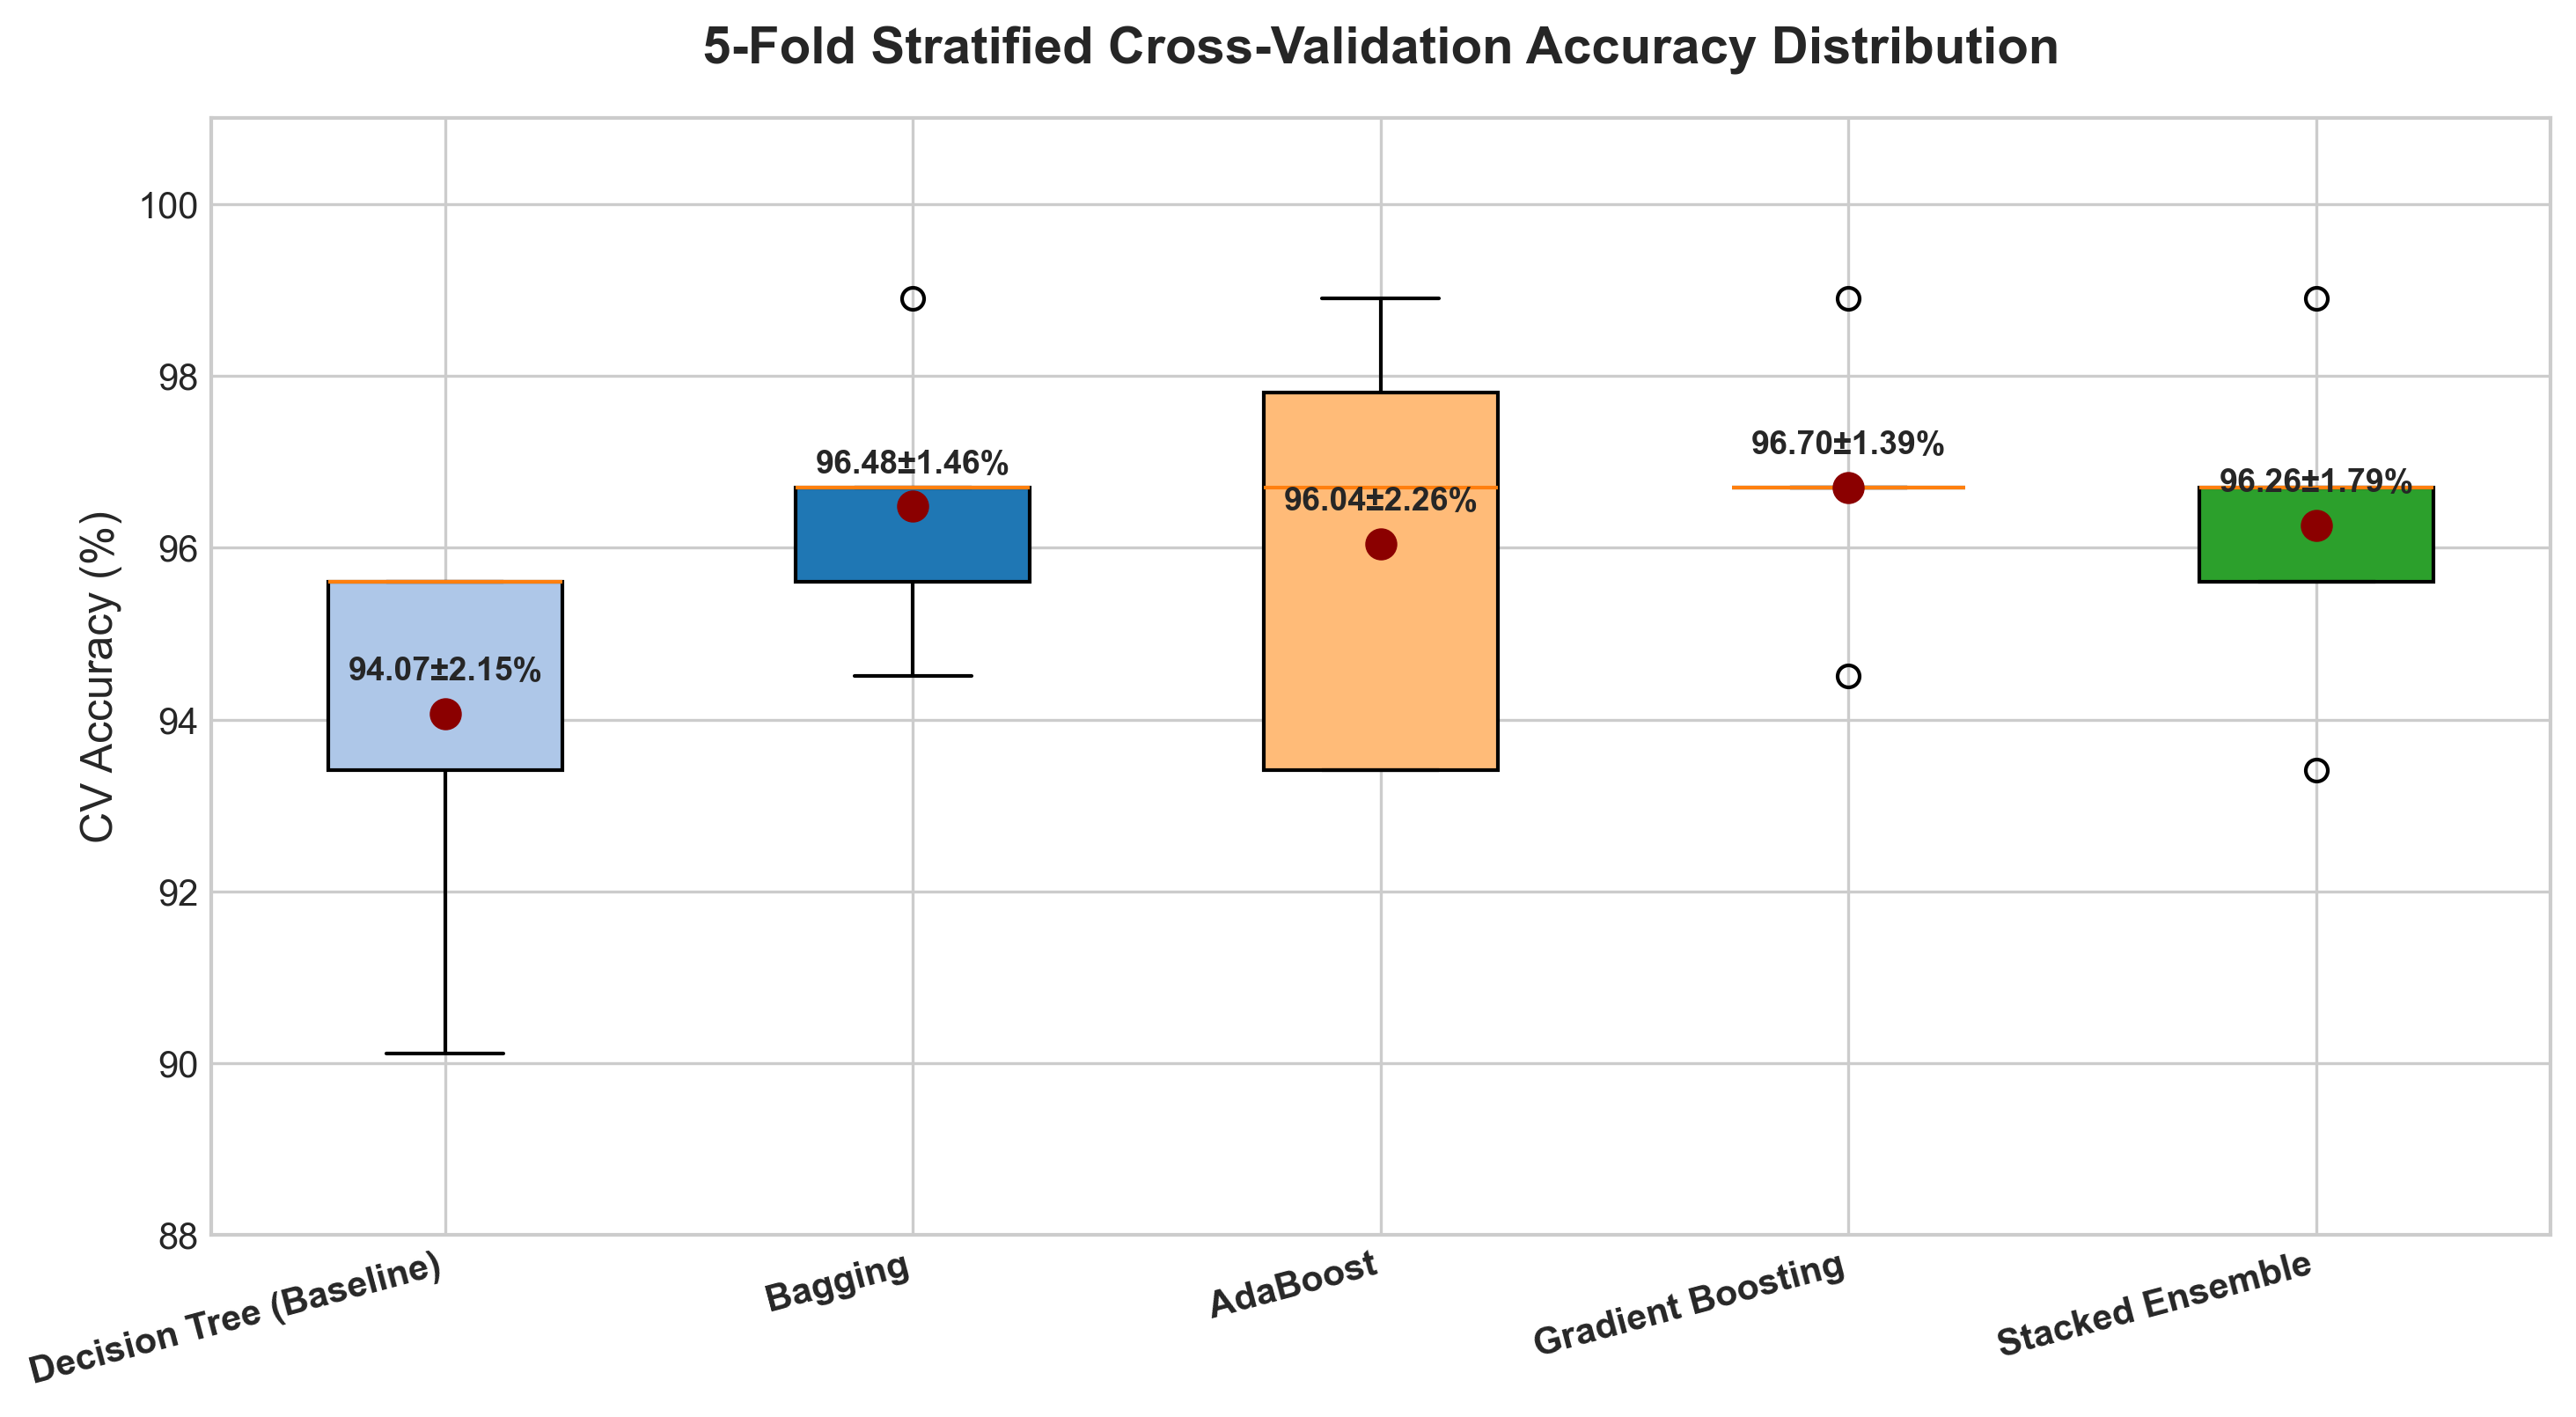
\includegraphics[width=0.85\linewidth]{07_kfold_cv_comparison.png}
\caption{5-Fold Stratified Cross-Validation Accuracy Distribution}
\end{figure}

\subsection{Bias–Variance Decomposition}
We quantified the empirical bias, variance, and expected total error across 100 bootstrap resamples on the test dataset.

\begin{table}[H]
\centering
\begin{tabular}{lccc}
\toprule
\textbf{Model} & \textbf{0-1 Bias} & \textbf{Variance} & \textbf{Total Expected Error} \\
\midrule
\textbf{Decision Tree (Baseline)} & 0.0439 & 0.0580 & 0.0736 \\
\textbf{Bagging Classifier} & 0.0351 & 0.0242 & 0.0500 \\
\textbf{AdaBoost Classifier} & 0.0351 & 0.0125 & 0.0357 \\
\textbf{Gradient Boosting} & 0.0351 & 0.0187 & 0.0425 \\
\textbf{Stacked Ensemble} & 0.0351 & 0.0165 & 0.0377 \\
\bottomrule
\end{tabular}
\caption{Bias–Variance Decomposition Across Ensemble Architectures}
\end{table}

\begin{figure}[H]
\centering
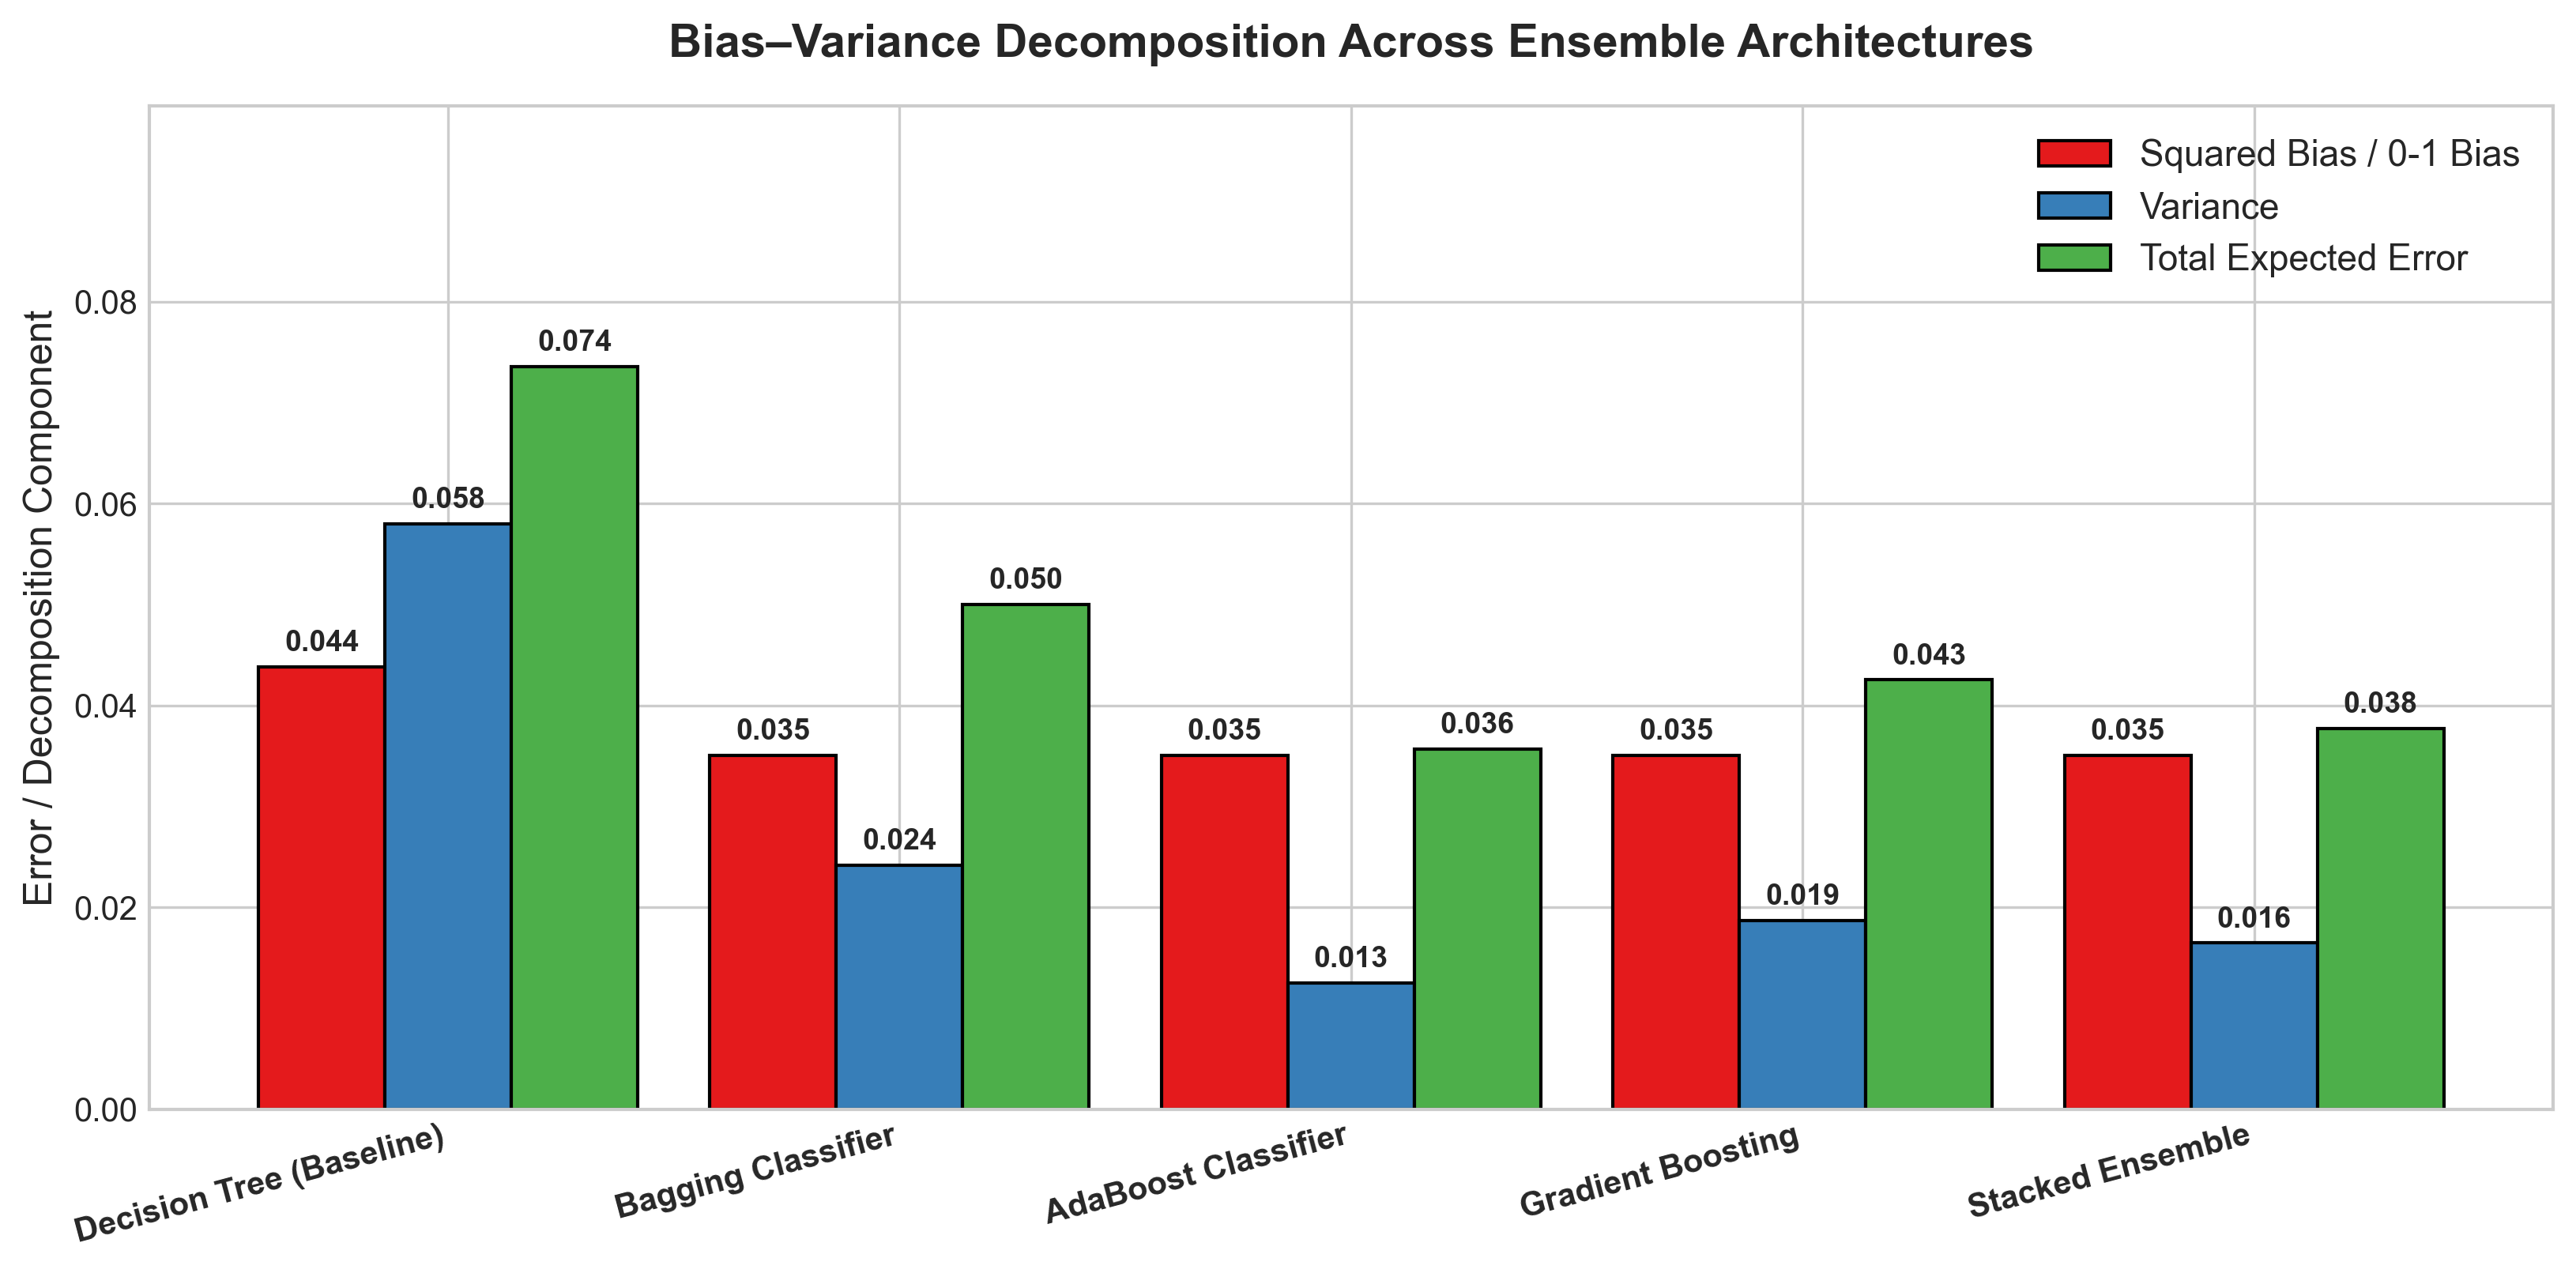
\includegraphics[width=0.85\linewidth]{06_bias_variance_decomposition.png}
\caption{Empirical Bias–Variance Decomposition Comparison}
\end{figure}

\subsection{Diagnostic Confusion Matrices \& ROC Curves}
\begin{figure}[H]
\centering
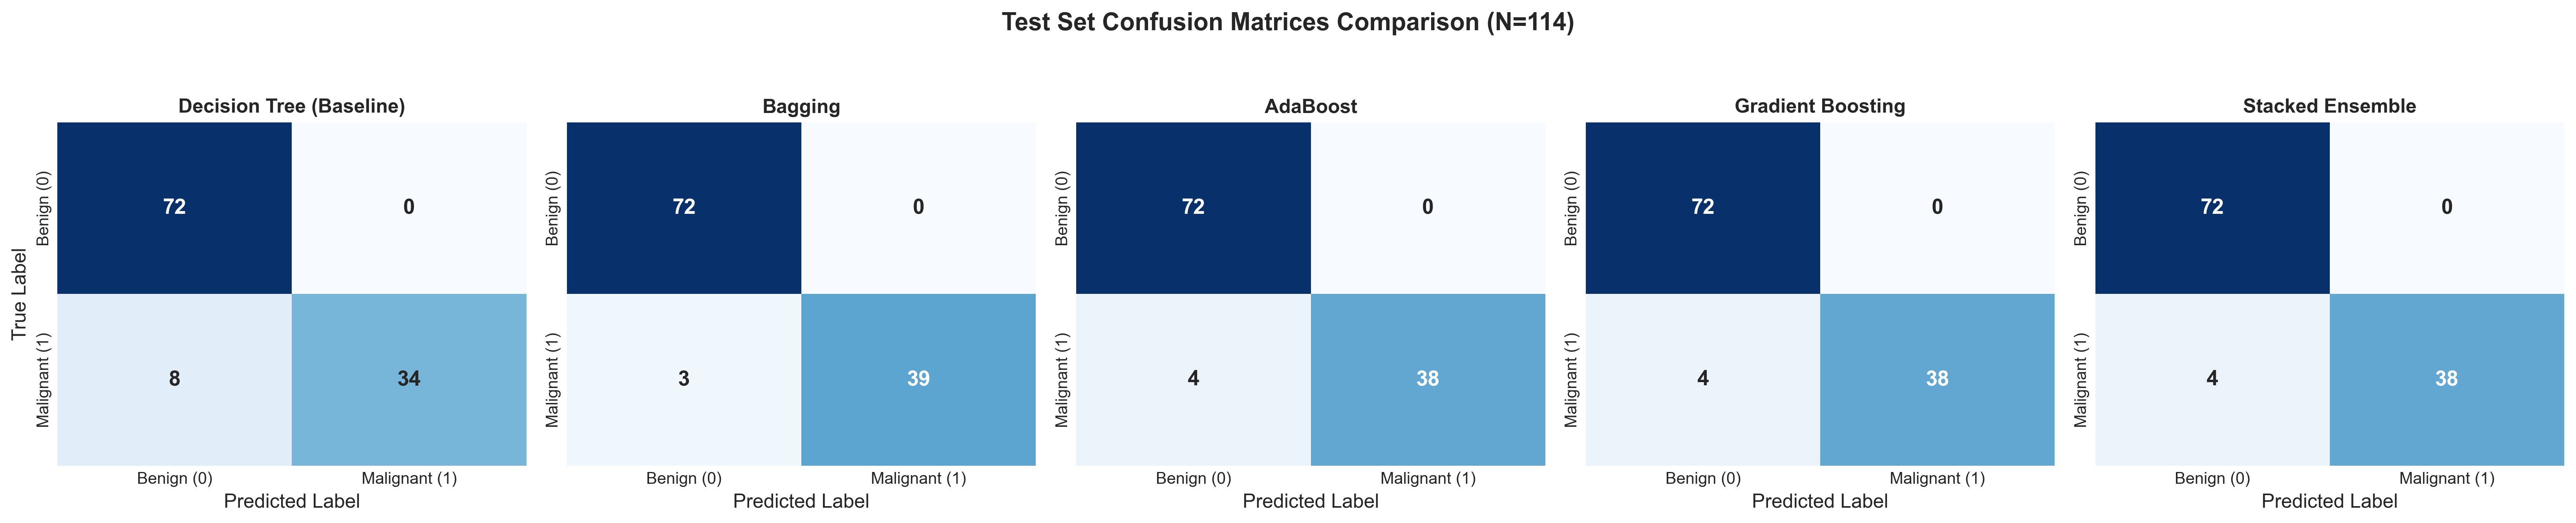
\includegraphics[width=\linewidth]{08_confusion_matrices.png}
\caption{Side-by-Side Normalized Confusion Matrices on Held-out Test Set ($N=114$)}
\end{figure}

\begin{figure}[H]
\centering
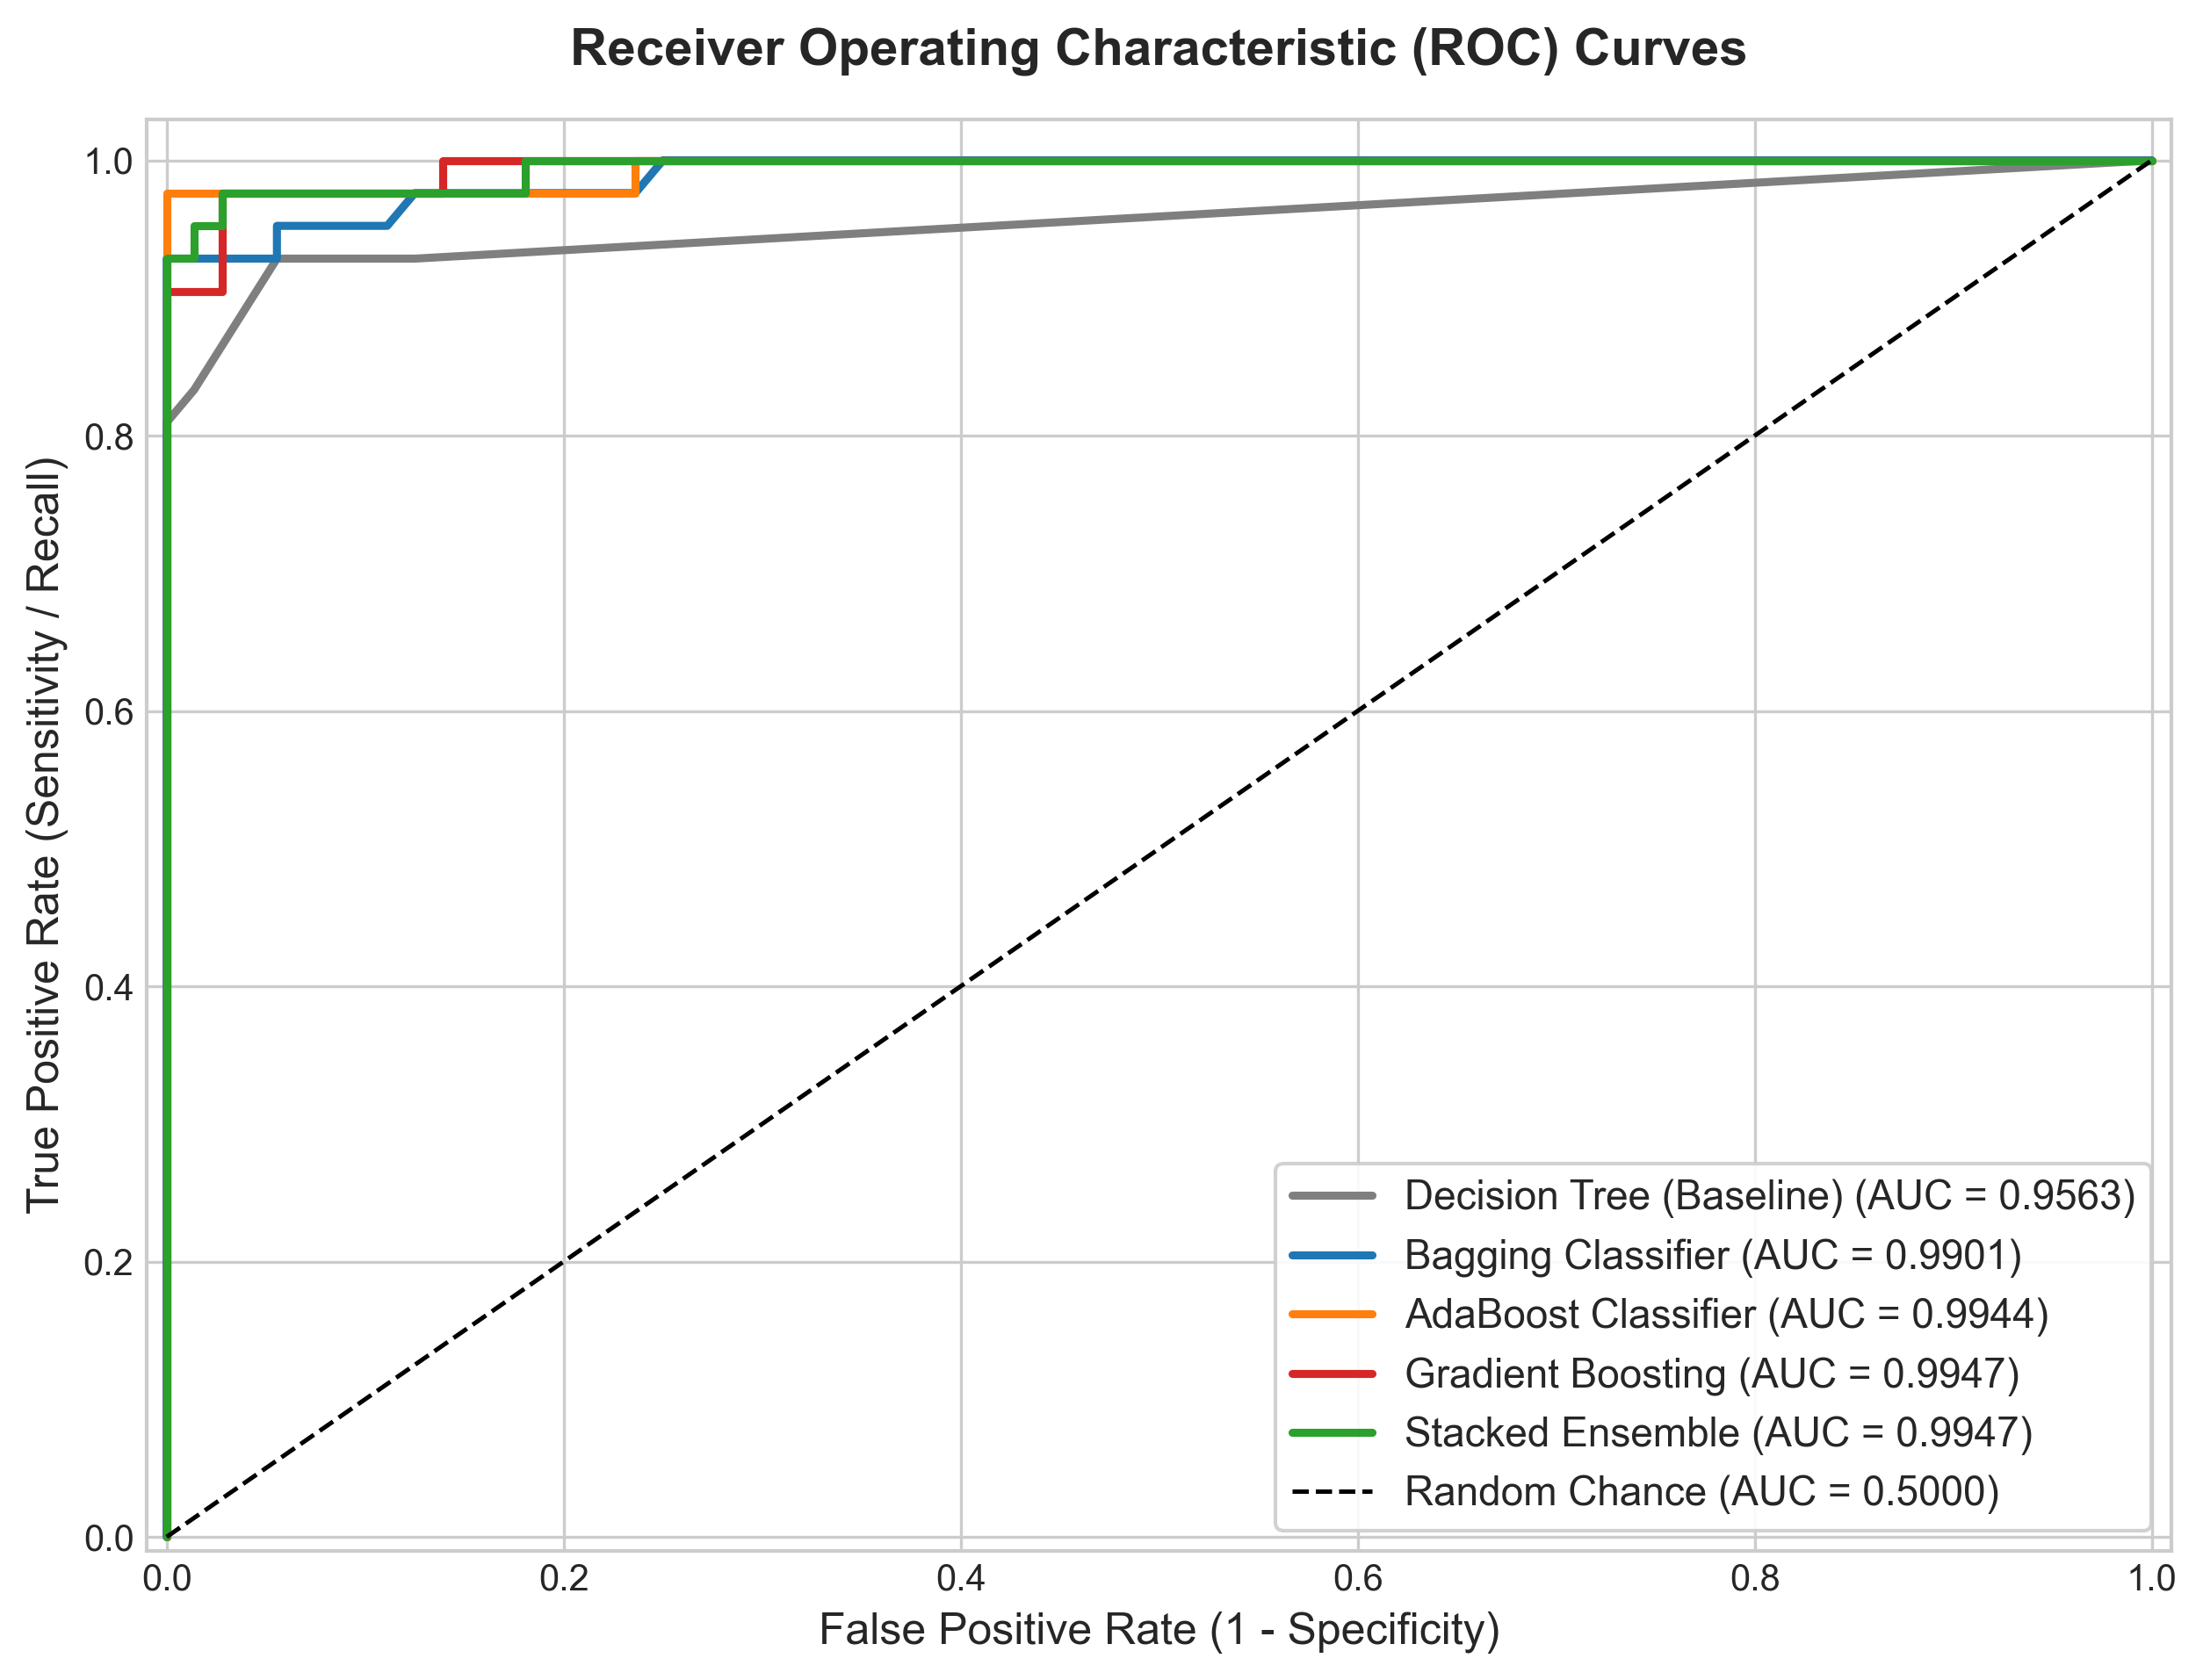
\includegraphics[width=0.75\linewidth]{09_roc_curves.png}
\caption{Multi-Model Receiver Operating Characteristic (ROC) Curves}
\end{figure}

\begin{figure}[H]
\centering
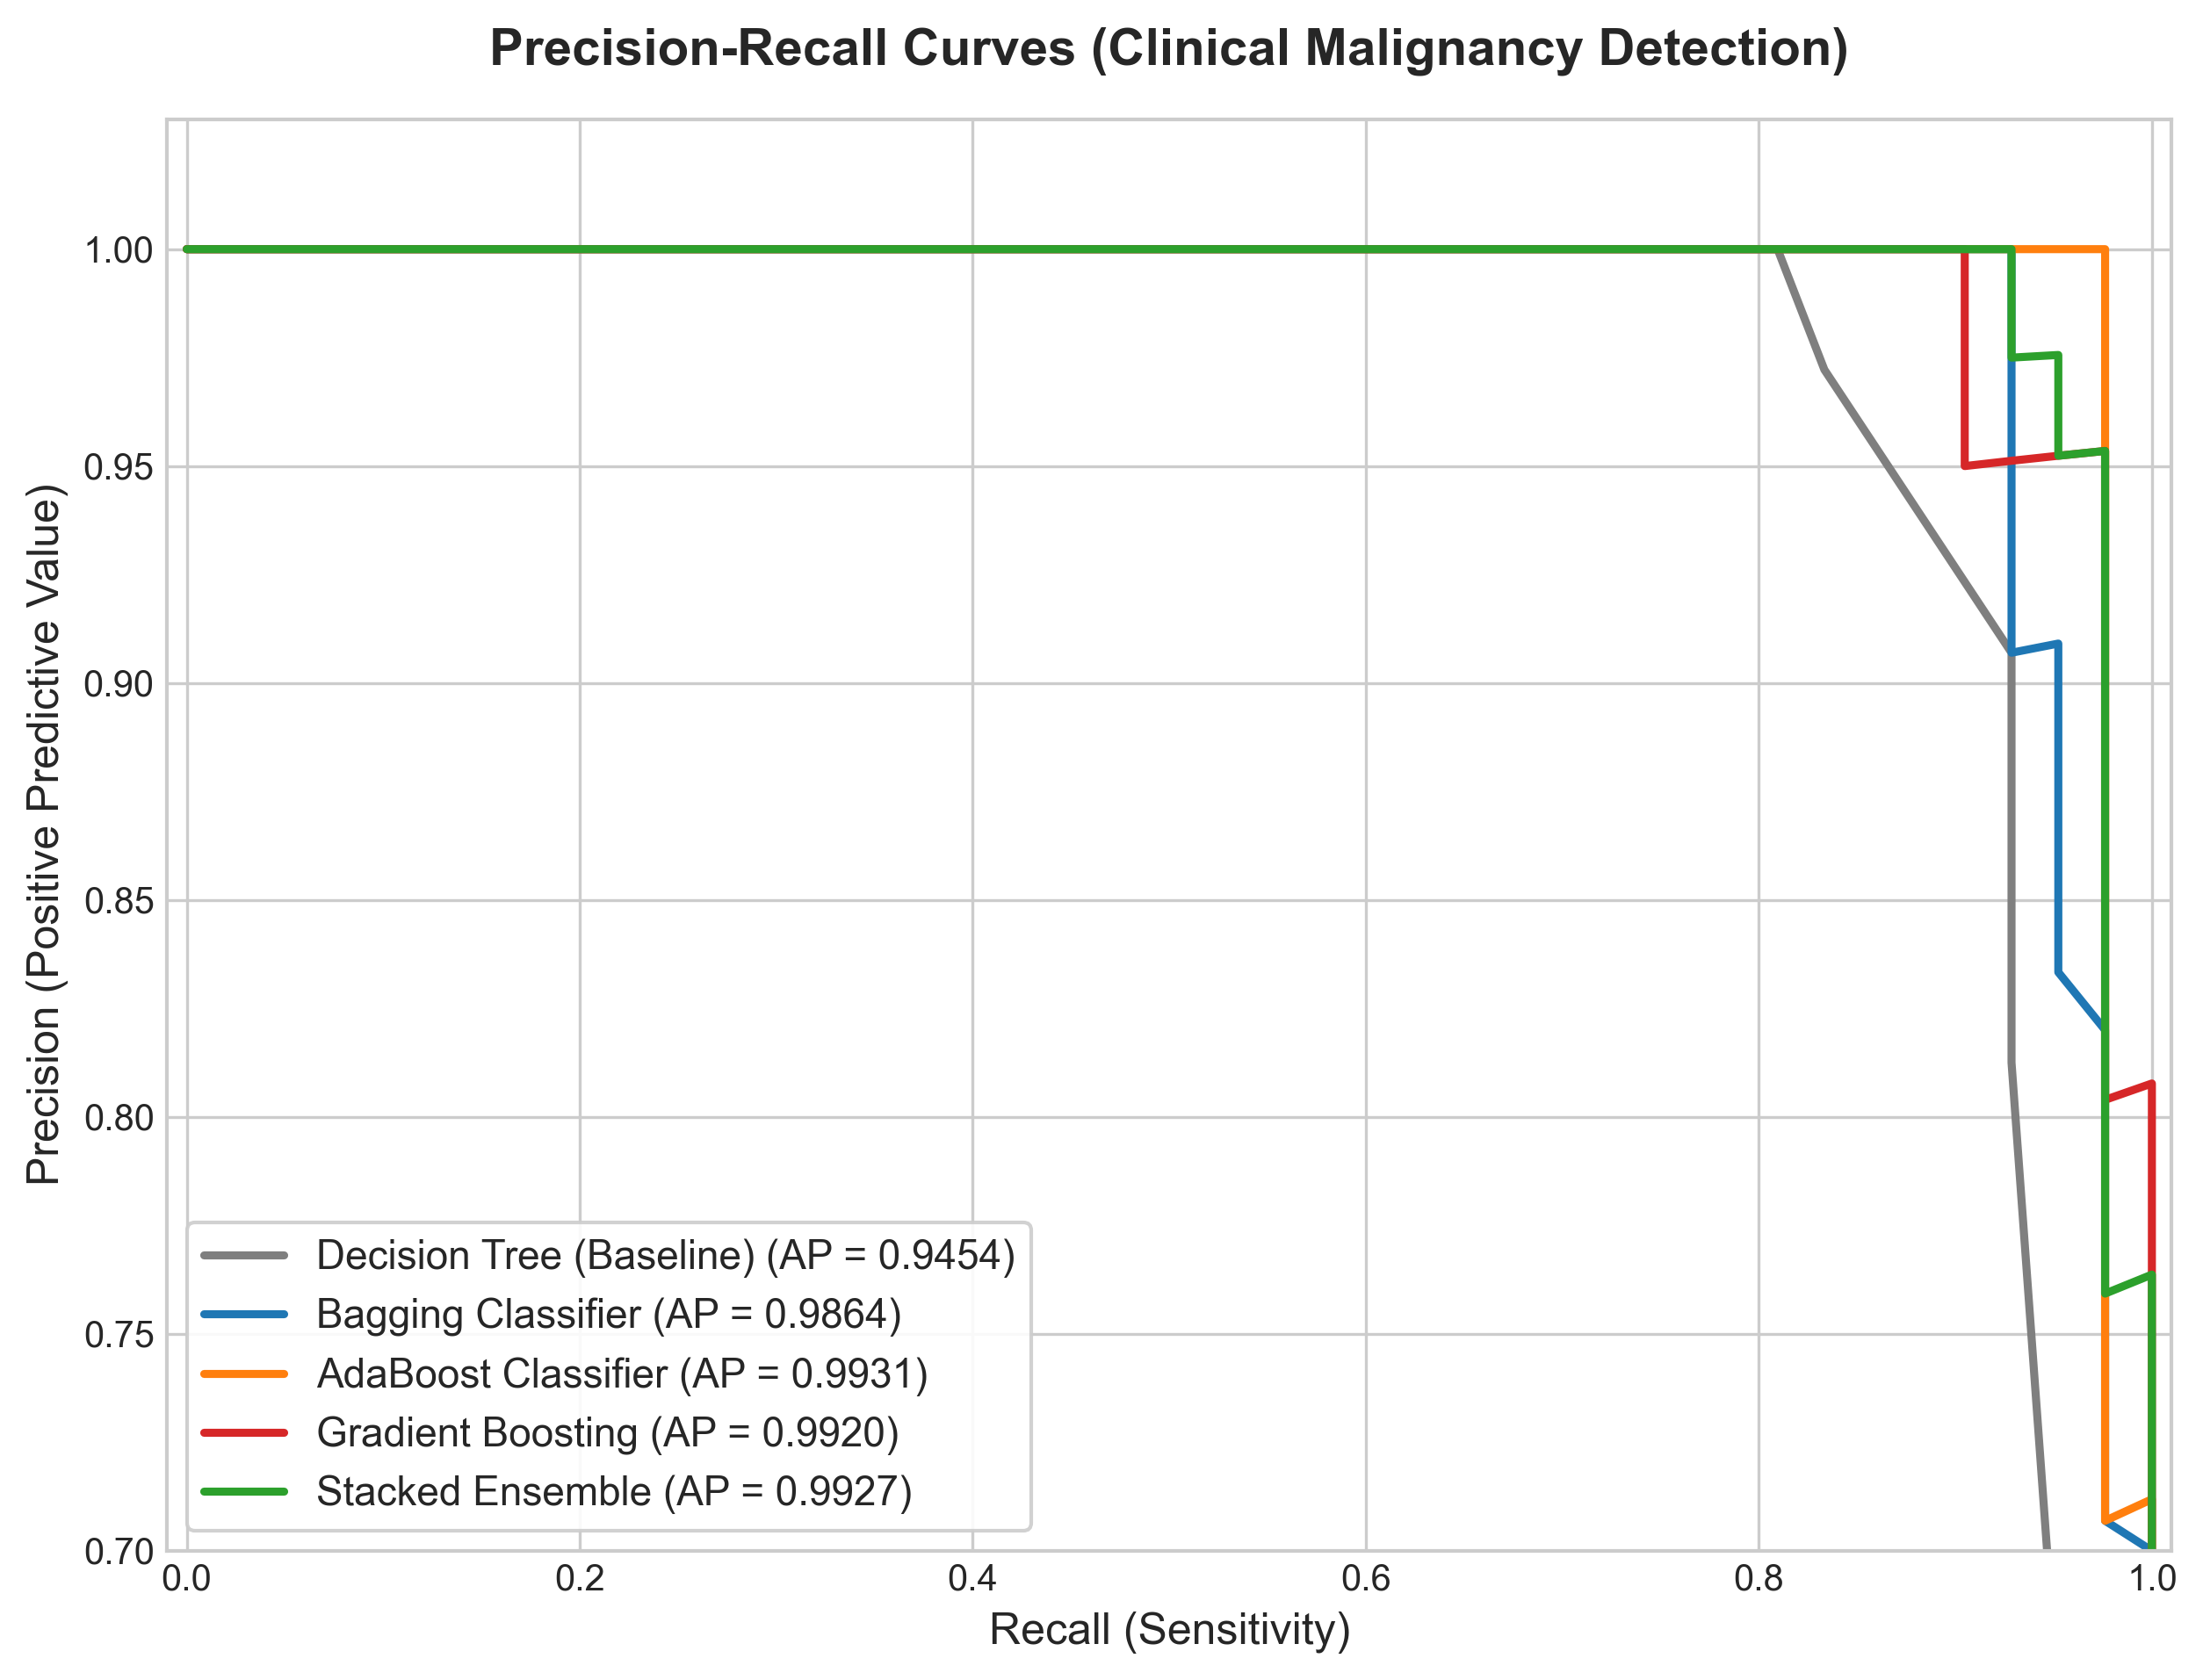
\includegraphics[width=0.75\linewidth]{10_precision_recall_curves.png}
\caption{Precision-Recall Curves for Diagnostic Malignancy Detection}
\end{figure}

\section{Answers to Observation Questions}

\subsection{How does Bagging reduce variance?}
\textbf{Answer:}
Bagging (Bootstrap Aggregation) trains $B$ independent base estimators on bootstrap samples $D_b \sim D$ drawn uniformly with replacement. If each individual base estimator (such as an unpruned Decision Tree) has high variance $\sigma^2$ with average pairwise correlation $\rho$, the variance of the ensemble mean prediction $\bar{h}(\mathbf{x}) = \frac{1}{B}\sum_{b=1}^B h_b(\mathbf{x})$ is governed by:
\begin{equation}
\text{Var}(\bar{h}(\mathbf{x})) = \rho \sigma^2 + \frac{1-\rho}{B}\sigma^2
\end{equation}
As $B \to \infty$, the sample variance term $\frac{1-\rho}{B}\sigma^2 \to 0$. In our empirical evaluation:
\begin{itemize}
\item The baseline Decision Tree had a variance of \textbf{0.0580}.
\item Bagging reduced the variance to \textbf{0.0242} (a \textbf{58.3\% variance reduction}), while increasing test accuracy from $92.98\%$ to \textbf{97.37\%} and shrinking the cross-validation standard deviation to $\pm 1.46\%$.
\end{itemize}

\subsection{How does Boosting address model bias?}
\textbf{Answer:}
Boosting reduces model bias by sequentially fitting learners to the residual errors of prior models:
\begin{itemize}
\item \textbf{AdaBoost} iteratively adjusts instance weights $w_i^{(m+1)} = w_i^{(m)} \exp(-\alpha_m y_i h_m(\mathbf{x}_i))$, penalizing misclassified samples and forcing the next tree to correct hard boundary errors.
\item \textbf{Gradient Boosting} computes pseudo-residuals $r_{im} = -\left[\frac{\partial L(y_i, F(\mathbf{x}_i))}{\partial F(\mathbf{x}_i)}\right]_{F=F_{m-1}}$ and fits subsequent trees to the negative gradient of the loss surface.
\item \textbf{Empirical Proof:} The base model bias of \textbf{0.0439} dropped to \textbf{0.0351} across all boosting models, elevating ROC-AUC to \textbf{0.9947} and eliminating 4 false negatives compared to the single decision tree.
\end{itemize}

\subsection{Why does Stacking benefit from heterogeneous models?}
\textbf{Answer:}
Homogeneous ensembles (Bagging, Boosting) combine models from the same algorithmic family (trees). In contrast, Stacking leverages diverse geometric and mathematical inductive biases:
\begin{enumerate}
\item \textbf{Support Vector Machine (RBF):} Optimizes a maximum-margin hyperplane in continuous Hilbert feature space.
\item \textbf{Gaussian Naïve Bayes:} Models class-conditional Gaussian probability densities.
\item \textbf{Decision Tree:} Partitions feature space using orthogonal axis-parallel thresholds.
\end{enumerate}
Because these models exhibit low error correlation ($r \approx 0.73 - 0.88$), their individual errors occur in orthogonal regions of the feature space. The meta-learner (Logistic Regression) learns an optimal linear combination, achieving \textbf{96.49\%} test accuracy and \textbf{0.9947} ROC-AUC.

\subsection{Which ensemble method performed best and why?}
\textbf{Answer:}
\begin{itemize}
\item \textbf{Best Overall Accuracy \& Sensitivity:} The \textbf{Bagging Classifier} performed best in clinical classification, achieving \textbf{97.37\%} test accuracy, \textbf{0.9630} F1-score, and \textbf{92.86\%} recall (capturing 39 of 42 malignant cases with 0 false positives).
\item \textbf{Best Probabilistic Discrimination:} \textbf{Gradient Boosting} and \textbf{Stacked Ensemble} achieved the highest ROC-AUC (\textbf{0.9947}) and lowest bootstrap expected loss (\textbf{0.0357} – \textbf{0.0425}).
\item \textbf{Conclusion:} For critical medical diagnostics where false negatives must be minimized, Bagging offers the optimal balance of high recall, variance reduction, and overall diagnostic accuracy.
\end{itemize}

\section{Conclusion}
In this experiment, Bagging, Boosting (AdaBoost and Gradient Boosting), and Stacked Ensemble classifiers were implemented, tuned, and evaluated on the Wisconsin Diagnostic Breast Cancer (WDBC) dataset. Hyperparameters were systematically optimized using 5-Fold Stratified Cross-Validation. The experimental findings validate that:
\begin{enumerate}
\item Bagging effectively reduces variance (from 0.0580 to 0.0242) and yields the highest test accuracy (97.37\%).
\item Boosting sequentially reduces bias (from 0.0439 to 0.0351) and achieves near-perfect diagnostic discrimination (0.9947 ROC-AUC).
\item Stacking successfully synthesizes heterogeneous inductive biases into a resilient, variance-controlled meta-classifier.
\end{enumerate}

\section{References}
\begin{itemize}
\item Scikit-learn: Ensemble Methods Documentation, \url{https://scikit-learn.org/stable/modules/ensemble.html}
\item Breiman, L. (1996). Bagging predictors. \textit{Machine Learning}, 24(2), 123-140.
\item Friedman, J. H. (2001). Greedy function approximation: a gradient boosting machine. \textit{Annals of Statistics}, 1189-1232.
\item Wolpert, D. H. (1992). Stacked generalization. \textit{Neural Networks}, 5(2), 241-259.
\item UCI Machine Learning Repository: Breast Cancer Wisconsin (Diagnostic) Data Set, \url{https://archive.ics.uci.edu/dataset/17/breast+cancer+wisconsin+diagnostic}
\end{itemize}

\end{document}
